\documentclass[a4paper,11pt]{article}

\setlength{\parindent}{0pt}

% Various packages
\usepackage{graphicx}
\usepackage{a4wide}
\usepackage{url}
\usepackage[left=2cm,top=2cm,bottom=1.5cm,right=2cm]{geometry}
\usepackage{amsmath}
\usepackage{amssymb}
\usepackage{amsthm}
\usepackage{amsfonts}
\usepackage{wrapfig}
\usepackage{fixme}
\usepackage{color}
\usepackage{pstricks}
\usepackage{pdfpages}
\usepackage[utf8]{inputenc}
\usepackage{enumitem}
\usepackage{tasks}
\usepackage{float}
\usepackage{dutchcal}

%\usepackage{minted}

\usepackage{listings}
\usepackage{lstautogobble}
\usepackage{semantic}

% Various custom commands
\newcommand{\argmin}{hrm{argmin}}
\newcommand{\R}{\mathbb{R}}
\newcommand{\E}{\mathbb{E}}
\newcommand{\mean}{\mathbb{E}}
\newcommand{\V}{\mathbb{V}}
\newcommand{\prob}{\mathbb{P}}
\newcommand{\var}{\mathrm{var}}
\newcommand{\iid}{\overset{\text{iid}}{\sim}}

\newcommand{\w}{{\mathbf w}}
\newcommand{\x}{{\mathbf x}}
\newcommand{\y}{{\mathbf y}}
\newcommand{\X}{{\mathbf X}}
\renewcommand{\P}[1]{\mathbb P\lrc{#1}}
\DeclareMathAlphabet{\mathpzc}{OT1}{pzc}{m}{it}

\newcommand{\lr}[1]{\left (#1\right)}
\newcommand{\lrc}[1]{{\left \{#1\right\}}}
\newcommand{\lra}[1]{\left |#1\right|}
\newcommand{\lrs}[1]{\left [#1\right]}


\lstset{basicstyle=\ttfamily,
  mathescape=true,
  escapeinside=||,
  autogobble}

\makeatletter
\newcommand*\bigcdot{\mathpalette\bigcdot@{.5}}
\newcommand*\bigcdot@[2]{\mathbin{\vcenter{\hbox{\scalebox{#2}{$\m@th#1\bullet$}}}}}
\makeatother
\usepackage{geometry}
\geometry{
  top=1.3in,    
  inner=1.4in,
  outer=1.4in,
  bottom=1.3in,
  headheight=3ex,  
  headsep=3ex,     
}
\usepackage{fancyhdr}
\pagestyle{fancyplain}
\pagestyle{fancy}
\fancyhf{}
\fancyhead[LE,RO]{Matilde Broløs}
\fancyhead[RE,LO]{PLD - Assignment 4}
\fancyfoot[CE,CO]{}
\fancyfoot[LE,RO]{\thepage}
\renewcommand{\plainheadrulewidth}{0.4pt}

%\usepackage{tikz}


% Making itemized lists that save space
\newenvironment{packed_itemize}{
\begin{itemize}
  \setlength{\itemsep}{1pt}
  \setlength{\parskip}{0pt}
  \setlength{\parsep}{0pt}
}{\end{itemize}}


\title{PLD Assignment 4}
\author{Matilde Broløs (jtw868)}
\date{\today}

\begin{document}

\maketitle

\section*{The Common Part}

\subsection*{A4C.1}
The statement for adding local variables
$$\texttt{local } \textbf{var } \texttt{in } \textit{Stat}$$
creates a new variable in the statement, and the variable is instantiated to $0$. To get the inverse of this, we need to assure that the inverse operations are performed, to ensure that tho local variable returns to the value $0$. That is, the inverse of the statement is
$$\texttt{local } \textbf{var } \texttt{in } \textit{Stat'}$$
where \textit{Stat'} is the inverse of \textit{Stat}.

\subsection*{A4C.2}
A gcd procedure does not output garbage in every iteration is shown below.

\begin{verbatim}
read m;
read n;

gcd()
  local g in
    if (n == 0)
      g += m;
      write g
    else
      g += m mod n
      m <-> n
      g <-> n
      gcd()
      g <-> n
      m <-> n
      g -= m mod n
    fi (n == 0)

gcd()

write m;
write n
\end{verbatim}

This procedure first reads m and n, then calls the function \texttt{gcd()}. This function creates a local variable \texttt{g} and then performs the same check as the repeat-loop in the procedure from figure 13.6 in "Programming Language Design and Implementation". If \texttt{n} is equal to zero, this means the greatest common divisor is the value of \texttt{m}, and therefore \texttt{g}, which is currently $0$, has \texttt{m} added to its value and is written. If \texttt{n} is not equal to zero, we perform the same operations as in the repeat-loop, then call \texttt{gcd()} recursively, and then performs the inverse operations to go back to the original values of the variables.

\subsection*{A4C.3}
The gcd program written in Python looks as follows.

\begin{verbatim}
m = int(input())
n = int(input())

def swap(x,y):
  a = x
  x = y
  y = a
  return x,y

def gcd():
  global m
  global n
  g = 0
  if (n == 0):
    g += m
    print(g)
    g = 0
    assert(n==0)
  else:
    g += m % n
    m,n = swap(m,n)
    g,n = swap(g,n)
    gcd()
    g,n = swap(g,n)
    m,n = swap(m,n)
    assert(n!=0)
  
gcd()  

print(m)
m = 0
print(n)
n = 0
\end{verbatim}


\section*{Option 3: Type and dictionary inference using logic programming}

\subsection*{A4O3.1}
The states about types in Haskell can be written in Pure Prolog as follows.

\begin{verbatim}
isDictOf(eqInt, eq(int)).
isDictOf(ordInt, ord(int)).

isDictOf(ordBool(X), ord(bool)) :-
  isDictOf(X,ord(int)).

isDictOf(optimizedOrd, ord(prod(int, int))).

isDictOf(ordPair(X,Y), ord(prod(A,B))) :-
  isDictOf(X, ord(A)),
  isDictOf(Y, ord(B)).

isTypeOf(qsortPrime(D,L), list(A)) :-
  isDictOf(D, ord(A)),
  isTypeOf(L, list(A)).
\end{verbatim}

I have chosen to use \texttt{isDictOf(A,B)} to represent the relationship that \texttt{A} is a dictionary of type \texttt{B}, and \texttt{isTypeOf(A,B)} to show that \texttt{A} is of type \texttt{B}.

\subsection*{A4O3.2}
To use Prolog to find all the dictionaries that can be passed to \texttt{qsort'} in the different cases, I add the following facts to implement the needed type in the program.

\begin{verbatim}
isTypeOf(list(A),list(A)).

isTypeOf(true,bool).
isTypeOf(false,bool).

isTypeOf(int,int).
\end{verbatim}

Now lets determine the number of dictionaries that can be passed to \texttt{qsort'} by running the quries seen in figure \ref{fig:dicts}.

\begin{figure}[h]
\centering
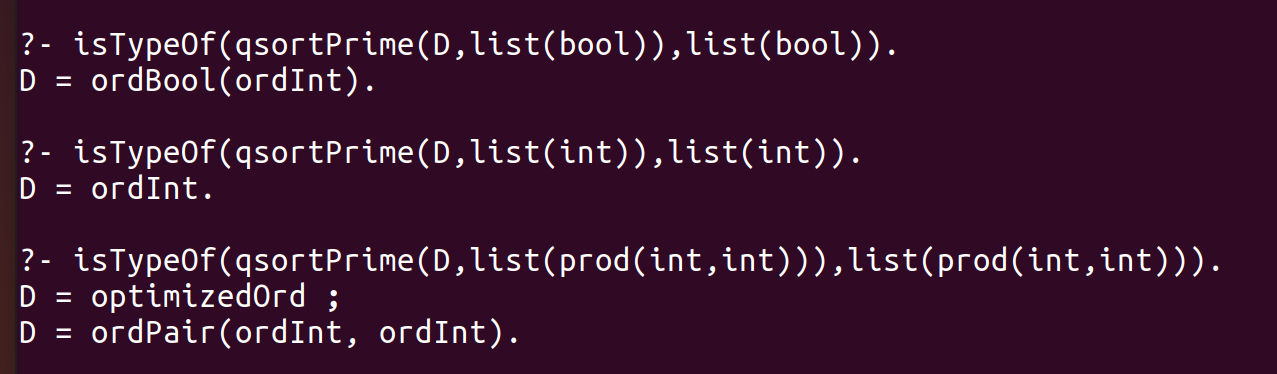
\includegraphics[width=0.8\textwidth]{O32.png}
\caption{Finding dictionaries to be passed to \texttt{qsort'}.}
\label{fig:dicts}
\end{figure}
\newpage
Thus there is one dictionary for boolean lists, one for integer lists, and two for lists of pairs of integers.

Now lets look at the resolution tree for the last query. By using the \textit{trace} command in SWI-Prolog, we can determine the way the program issues the query. This is seen in figure \ref{fig:resTrace}.

\begin{figure}[h]
\centering
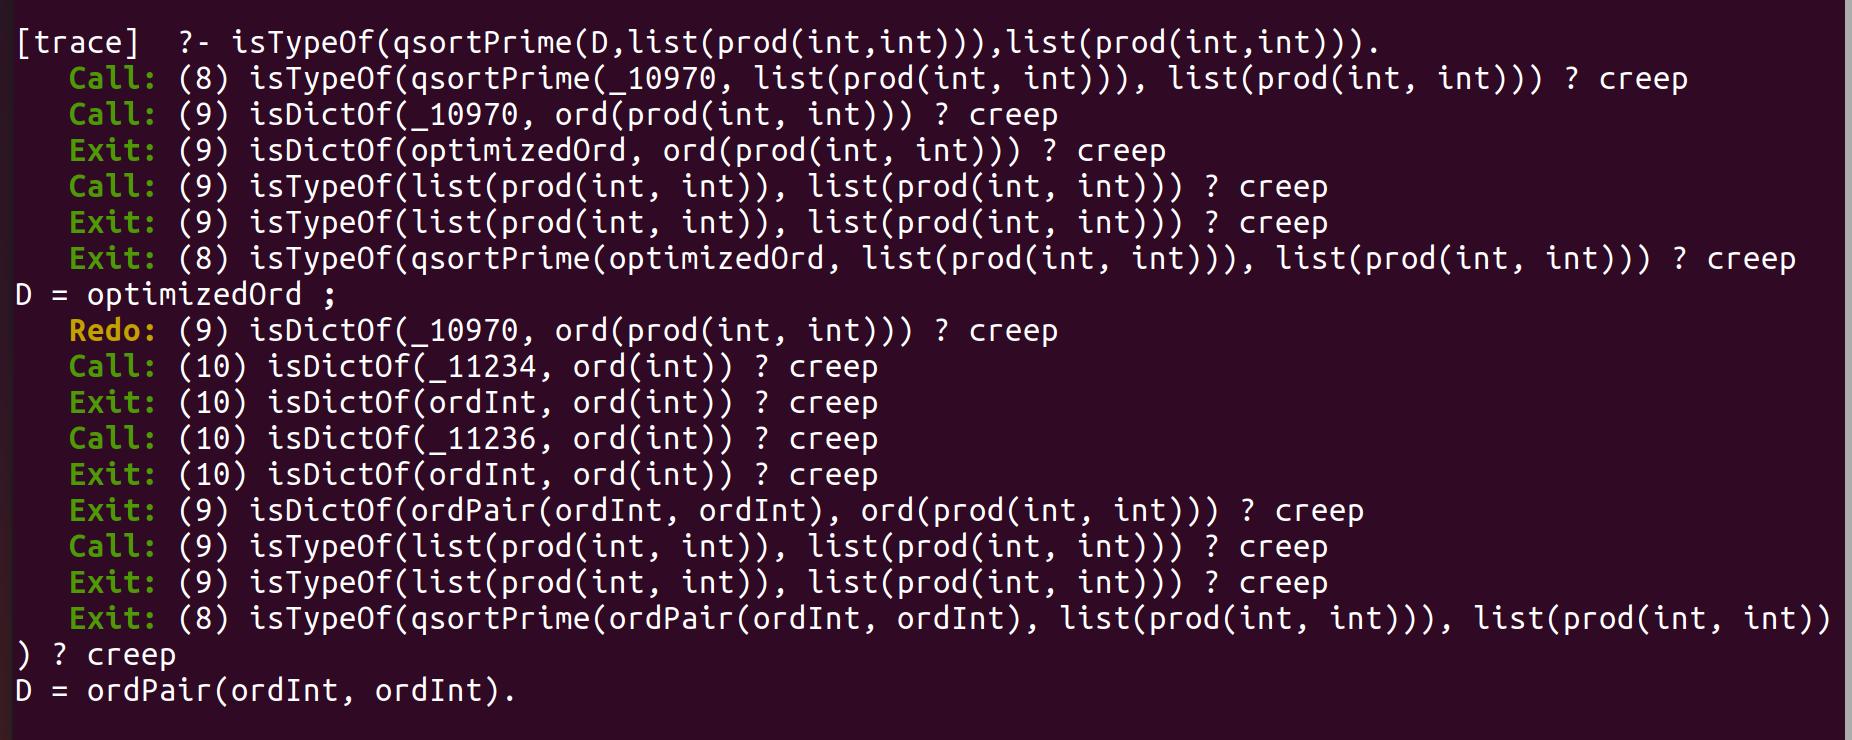
\includegraphics[width=0.8\textwidth]{resTrace.png}
\caption{The result of running the query while \textit{trace} is active.}
\label{fig:resTrace}
\end{figure}

From this the resolution tree shown in figure \ref{fig:resTree} is drawn.

\begin{figure}[h]
\centering
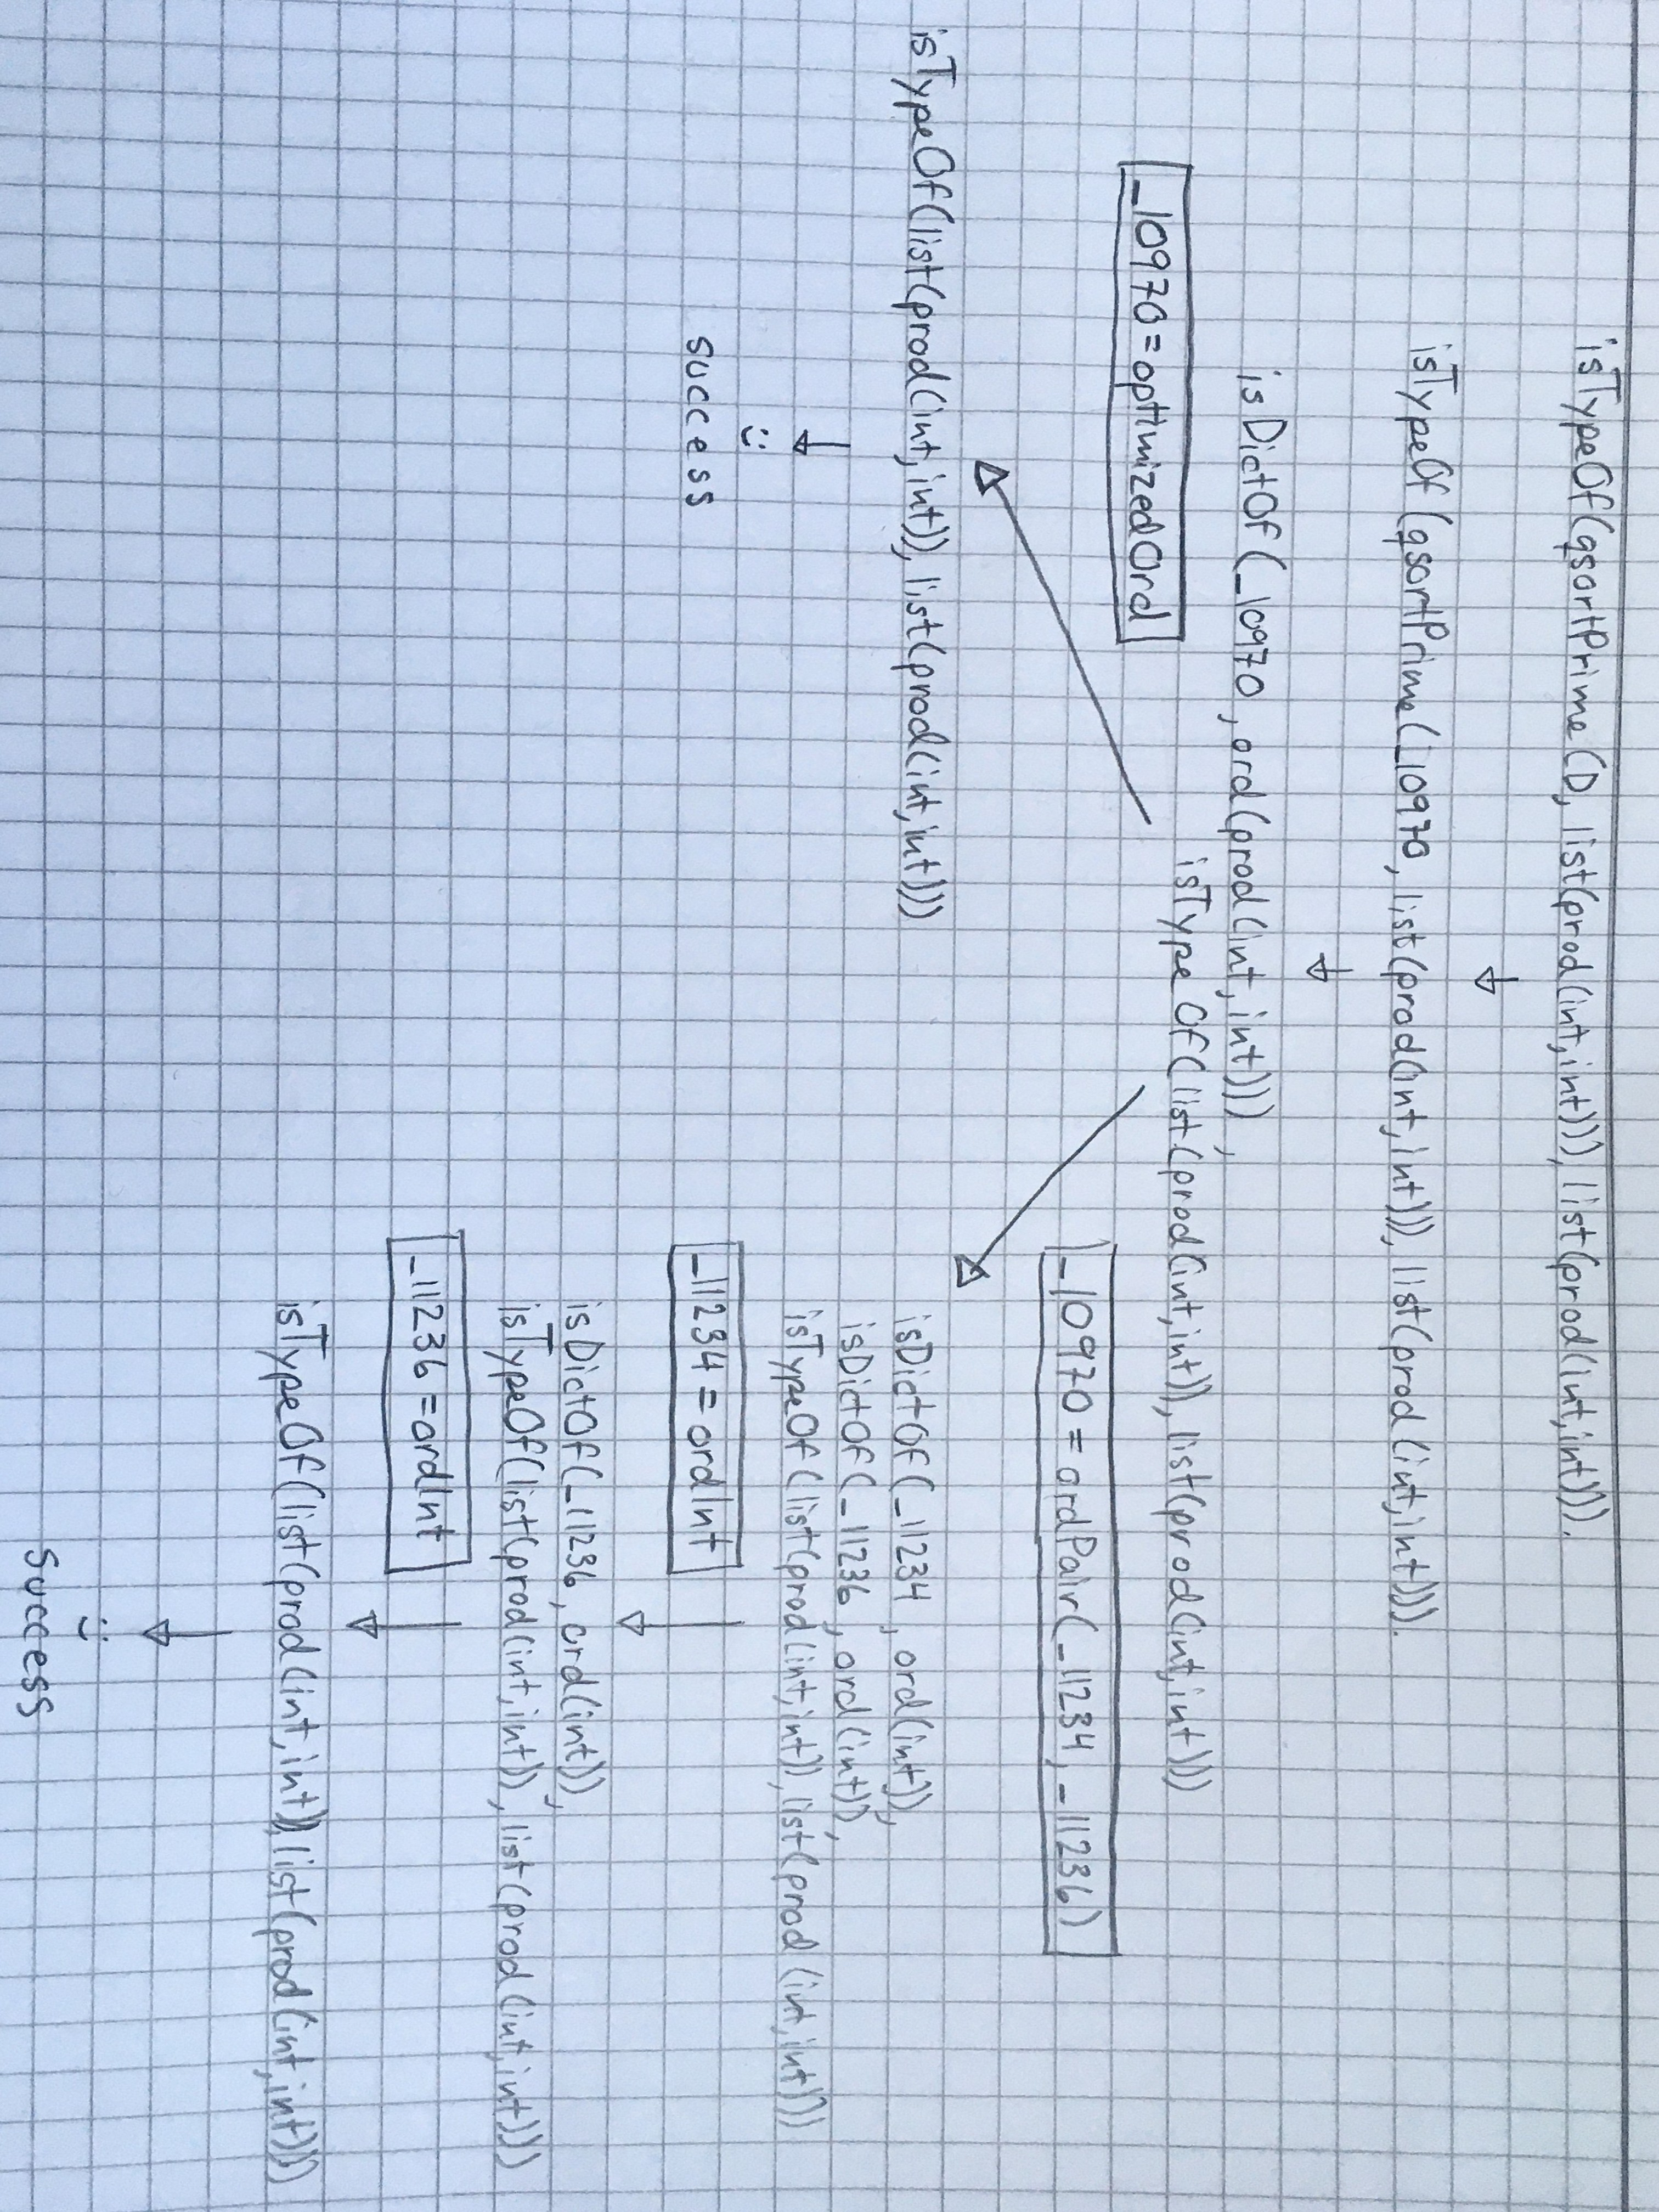
\includegraphics[width=0.8\textwidth]{resTree.jpg}
\caption{The resolution tree for the query.}
\label{fig:resTree}
\end{figure}

\newpage
\subsection*{A4O3.3}
The rules for subtyping was added by the following Prolog facts and implications.

\begin{verbatim}
isTypeOf(X,B) :-
  isSubtypeOf(A,B),
  isTypeOf(X,A).


isSubtypeOf(bool,int).

isSubtypeOf(list(A),list(B)) :-
  isSubtypeOf(A,B).

/*
isSubtypeOf(A,C) :-
  isSubtypeOf(A,B),
  isSubtypeOf(B,C).
*/
\end{verbatim}
The last one is out commented as it produces an infinite loop, and since we will not need it we will just leave it out commented. The reason for the infinite loop is that when asking what dictionaries we can pass to \texttt{qsort} when sorting a list of booleans, outputting a list of integers, we first get one correct answer \texttt{ordInt}. Then we backtrack to try to find more solutions, and in that process we ask if \texttt{int} is a subtype of any type. We know it isn't, but because of the transitivity rule, the query will run infinitely, thus creating the infinite loop that prevents the program from terminating.

Now, in figure \ref{fig:boollist} is is determined how many different dictionaries that could be passed to \texttt{qsort'}, by issuing the following query.

\begin{figure}[h]
\centering
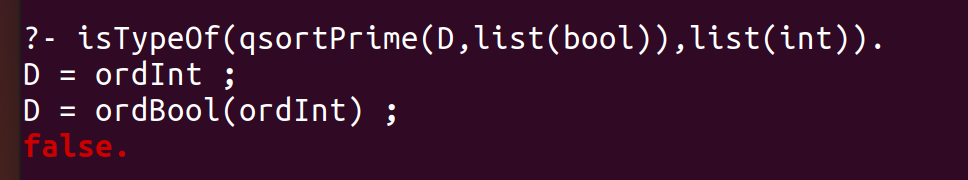
\includegraphics[width=0.8\textwidth]{O33.png}
\caption{Finding dictionaries for sorting a list of booleans into a list of ints.}
\label{fig:boollist}
\end{figure}

This means that there are two dictionaries that can be passed to \texttt{qsort'}. In this case both dictionaries work pefectly fine for sorting the list, but what if we didn't know whether we had a list of booleans or a list of integers? Then it might be smartest for us to use the \texttt{ordInt} dictionary, as that dictionary can sort both integers and booleans, and thus it is the more general dictionary of the two. Thus the dictionary the compiler should choose would be \texttt{ordInt}.

\subsection*{A4O3.4}

\subsubsection*{\textbf{(a)}}
The following code snippet shows how \textbf{cuts} can be added to the facts and implications for O3.1 to ensure that only one dictionary of each type is found.

\begin{verbatim}
isDictOf(eqInt, eq(int)) :- !.
isDictOf(ordInt, ord(int)) :- !.

isDictOf(ordBool(X), ord(bool)) :-
  isDictOf(X,ord(int)),
  !.

isDictOf(optimizedOrd, ord(prod(int, int))) :- !.

isDictOf(ordPair(X,Y), ord(prod(A,B))) :-
  isDictOf(X, ord(A)),
  isDictOf(Y, ord(B)),
  !.
\end{verbatim}

By adding these cuts, the query \texttt{isDictOf(X,ord(prod(int,int)))} will output only \texttt{optimizedOrd} instead of both \texttt{optimizedOrd} and \texttt{ordPair(ordInt,ordInt)}.

Here I use the method of adding a cut in the end of each fact and predicate, as this will ensure that if there has been found one dictionary of a type, the query will end. This is not nessecarily a very neat way to ensure this, and it results in always choosing the dictionary of a certain type which is declared first in the program. Therefore, the author should maybe put some thought into the order in which the program is written. For example, is it desirable to get the most specific dictionary, or the most general? That is something that should be consideres when ordering the facts and implications.

The con of this way of choosing a specific dictionary is, that the program will choose for you, and if you are not aware that your code is ambiguous, you will never know and thus never really get to choose for yourself.


\subsubsection*{\textbf{(b)}}
If we want to check wether there are several dictionaries of the same type, eg. \texttt{A}, we can in Prolog perform the query \texttt{isDictOf(X, A)}, and it will output all instances and conditional instances of that type - unles of course you have added cuts. Using this idea, it would be possible to check every type of dictionary manually, to determine whether multiple dictionaries of that type existed. However this would have to be done manually, or at least all types of dictionaries would have to be put in a list, so that we can loop through the list and check every type.

\subsection*{A4O3.5}
Programming languages using type inferrence allows the programmer to be more free when programming, not having to worry about types all the time. This could in general make writing code easier, as it makes the procedure of writing code less complicated, and might especially be well suited for people who are new to programming, or at least to a specific programming language. Type inferrence makes the learning curve less steep. \par
It is also convenient when not quite knowing what type a function will output, maybe because there are multiple possible types of putput. This let the programmer implement one single function or procedure for something that might have needed several functions if the type wasn't inferred. In "Programming Language Design and Implementation" section 8.1 we are given a conditional as an example. Here, different branches of the conditional could give different types for the answer. Here, type inferrence is convenient, as we can still have one combined conditional, even though the resulting types vary. \par
Furthermore, in the specific case of \texttt{qsort} it is practical that the compiler can itself infer what type of dictionary it needs for sorting a list, so that the programmer need not worry about this, as it would probably not enhance the programmers understanding of the program, but would only slow the programmer down.\par

However, type inferrence can also make the code more difficult to understand, and less clear, as the programmer is not forced to have an overview of the types of the program. This often helps a progremmer think his or her programs through, and thus causes the programmer to make less errors. On top of this, it also means more work for the compiler, as it needs to perform all this type inferrence instead of letting the programmer do it.\par
And even though type inferrence makes the learning curve of a programming language less steep, it sometimes also prevents the programmer from truly writing good programs. Take for example C - when you first start learning it it might seem very difficult and hard to understand intuitively, but when you get good at it it might actually give you more freedom than some other programming languages.\par

A combination where we get some advantages of type inferrence, without getting the disadvantages, could be an example where the compiler infers the type whenever it is possible. Whenever types are ambiguous the compiler could produce an error, forcing the programmer to make the code unambiguous. Using this combination, we both get to be lazy, but never lets the compiler choose for us.\par
Another combination could be \textit{soft typing}, as mentioned on page 154 in the notes. Soft typing never rejects programs as faulty, but instead uses dynamic type checking in the places where type inferrence is unamboguous. This can, according to the notes, be used as feedback for the programmer, and is often used for optimisation of dynamically typed languages.


\end{document}
